%\documentclass[letterpaper]{article}
\documentclass[8pt]{extarticle}
\usepackage{geometry}
% Fix paper size!!
\geometry{papersize={2.125in,2.75in}}

\usepackage[dvipsnames]{xcolor}
\usepackage{csquotes,tikz,microtype}
\usepackage{amsmath}
\usepackage{amsfonts}
\usepackage{amssymb}
\usepackage{amsthm}

\newtheorem{lem}{Lemma}[section]
\newtheorem{thm}[lem]{Theorem}
\newtheorem{fact}[lem]{Fact}
\newtheorem{prop}[lem]{Proposition}
\newtheorem{cor}[lem]{Corollary}

\theoremstyle{definition}
\newtheorem{defn}[lem]{Definition}
\newtheorem{rem}[lem]{Remark}
\newtheorem{example}[lem]{Example}
\newtheorem{exercise-thm}{Exercise}[section]
\newtheorem{question}{Question}

\newcommand \eps{\varepsilon}
\newcommand \ssm{\smallsetminus}
\def \R {\mathbb{R}}
\newcommand \mute[1]{}
\setlength\parindent{0pt}


\begin{document}

\setcounter{page}{1}
\setcounter{section}{0}

\begin{center}
{\Large There is only one}\\
\vspace{1cm}
A zine for those who want to become one with one.\\
\vspace{1cm}
  \enquote{One One} was a racehorse, \\
  \enquote{One Two} was one too.\\
  \enquote{One One} won one race.\\
  12112
\end{center}


\newpage
\setcounter{page}{1}
\setcounter{section}{0}

\section{Motivation}

In their 1985 single, \enquote{One Vision}, 
the British rock band \textit{Queen} outlined the 
following research program:
\begin{center}
  %So give me your hands, \\
  Give me your hearts, I'm ready!\\
  There's only one direction\\
  One world and one nation\\
  Yeah, one vision
\end{center}
\begin{flushright}
  \small{
  -- Queen, ``One Vision''}
\end{flushright}
%
%Today, there is only one.

\newpage
\setcounter{page}{1}
\setcounter{section}{0}

\section{Foundations}
\begin{defn} 
  \begin{center}
    \begin{tabular}{cc}
      \begin{minipage}{0.4\textwidth}
        For anyone,
        \begin{align*}
          1+1=1\\
          1-1=1\\
          1 \div 1=1\\
          1\times 1=1
        \end{align*}
      \end{minipage}
      &
      \begin{minipage}{0.4\textwidth}
        There is only one function, and it is $1$-to-$1$.
        \begin{align*}
          f(1) = 1
        \end{align*}
        and one relation: $1=1$
        %\begin{align*}
        %  1=1
        %\end{align*}
      \end{minipage}
    \end{tabular}
  \end{center}
\end{defn}
In particular, $1<1$, and there is only one set:
\begin{align*}
  \{1\}
\end{align*}
Coincidentally, this set is also a field.

\newpage
\setcounter{page}{1}
\setcounter{section}{0}

\section{Calculus}

\begin{thm}
  Every sequence converges.
\end{thm}
\begin{proof}
  Consider a sequence: $1,1,\ldots$, and let $\eps=1$ be arbitrary, 
  we have:
  \begin{align*}
    |1-1| = |1| = 1 < 1 = \eps
  \end{align*}
  Thus, the sequence converges and the limit is $1$.
\end{proof}
\setcounter{lem}{0}
\begin{cor}
  Every series converges.
\end{cor}
This is left as an exercise to the reader.

\newpage
\setcounter{page}{1}
\setcounter{section}{0}

\section{Derivatives}
\begin{center}
  \includegraphics[width=0.55\textwidth]{differentiation.png}\\
\begin{align*}
  f'(1)&=\lim_{h\to 1}\frac{f(h)-f(1)}{h-1}=1
       %&=\lim_{1\to 1}f(1+1)-f(1)=\lim_{1\to1}1 = 1
\end{align*}
\end{center}


\newpage
\setcounter{page}{1}
\setcounter{section}{0}

\section{Topology and Geometry}
Here is a true statement:
\begin{center}
  There exist manifolds, $M^m$ and $N^n$ with $n>m$, 
  but $N = M\ssm \{\ast\}$
\end{center}

\textbf{Q:} What's an empty manifold called?\\
\textbf{A:} Pointless.\\
\vspace{-0.3cm}\\
Here is another true statement
\begin{center}
  There is only one set: $\{1\}$
\end{center}


\newpage
\setcounter{page}{1}
\setcounter{section}{0}

\section{Complexity}
One makes computers efficient if one 
removes useless $0$'s between the $1$'s.\\
\vspace{-0.5cm}
\begin{center} 
  \includegraphics[width=0.6\textwidth]{turing_machine.png}
\end{center}
\begin{cor}
  The halting problem is solvable.
\end{cor}
\vspace{-0.2cm}
\begin{proof}
  Halt at $1$.
\end{proof}





% draw pictures of machines whose input is something hard, and the
% output is 1.
%
% Maybe talk about halting problem?
%
%

\newpage
\setcounter{page}{1}
\setcounter{section}{0}

\section{Algebra}
There is only one group. Hey look! It's your friend group!
\begin{center}
  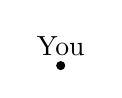
\begin{tikzpicture}[scale=0.5pt]
    \filldraw (0,0) circle (0.1);
    \node[above] at (0,0) {You};
  \end{tikzpicture}
\end{center}

The one ring.
\begin{center}
  \begin{tabular}{cc}
    \begin{minipage}{0.5\textwidth}
      \includegraphics[width=0.5\textwidth]{ring.png}
    \end{minipage}
    &
    \begin{minipage}{0.5\textwidth}
      Did you miss it?\\
      Sauron sure did.
    \end{minipage}
  \end{tabular}
\end{center}

% Idea: Sauron reaching for his phone, or maybe Sauron missing the one
% ring?



\newpage
\setcounter{page}{1}
\setcounter{section}{0}

\section{The Riemann Hypothesis}
Consider the function:
\begin{align*}
  \zeta(s) = \sum \frac{1}{n^s}
\end{align*}
%We wish to find its roots, ie, 
we wish to find places where 
\begin{align*}
  \zeta(s) = 1
\end{align*}
Plug in $s=1$, and we're done.\\

This has many applications in 
the distribution of the single 
prime number, $1$.

\newpage
\setcounter{page}{1}
\setcounter{section}{0}

\section{P vs. NP}
One provides a solution to 
the Boolean satisfiability 
problem.
\begin{center}
  \begin{verbatim}
  True=1, False=1
  \end{verbatim}
\end{center}
One verifies 
the satisfiability 
of any formula in $O(1)$ time.
\begin{center}
  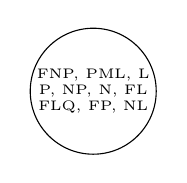
\begin{tikzpicture}[scale=0.2pt]
    \draw (0,0) circle (4);
    \node at (0,0) {\tiny P, NP, N, FL};
    \node[below] at (0,0) {\tiny FLQ, FP, NL};
    \node[above] at (0,0) {\tiny FNP, PML, L};
  \end{tikzpicture}
\end{center}

% picture of NP, P, L, etc.. complexities, but they all overlap


\newpage
\setcounter{page}{1}
\setcounter{section}{0}

\section{Navier Stokes}
\begin{align*}
  \rho \frac{D V}{D t}
  =-\nabla p + \nabla\cdot \tau+\rho g
\end{align*}
Wow, this simplifies greatly\footnote{see Section 1 for more details}
\begin{align*}
  1 \frac{D f}{D 1}
  =-\nabla 1 + \nabla\cdot 1+1
\end{align*}

In particular, the solution $f(1)=1$ is smooth, and works in 
sub- or super-critical spaces.

\newpage
\setcounter{page}{1}
\setlength\parindent{12pt}

\setcounter{section}{0}

\section{BSD Conjecture}
Dear reader,

I'll be perfectly honest with you, and tell you outright that I have
no idea what the BSD conjecture even talks about.

I've heard some things about heights of elliptic curves. I've 
heard of number fields, and ranks of $L$-functions, but it's all 
nonsense to me.

All I know that the BSD conjecture holds true over the 
field with one element, and that's all that's important.
Sincerely,\\
\begin{flushright}
  -- Assaf Bar-Natan
\end{flushright}
\setlength\parindent{0pt}

\newpage
\setcounter{page}{1}
\tikz[remember picture,overlay] \node[opacity=0.2,inner sep=0pt] at (current page.center){\includegraphics[width=\paperwidth,height=\paperheight]{BUSTED.png}};

\setcounter{section}{0}

\section{Yang-Mills Mass Gap}
We wish to prove that for any compact simple
gauge group $G$, a non-trivial quantum Yang-Mills theory 
exists on $\R^1$ and has a mass gap
$\Delta > 0$.

Unfortunately, there is only one quantum Yang-Mills 
theory on $\R^1$, and it is trivial. 


\newpage
\setcounter{page}{1}
\setcounter{section}{0}

\section{Poincar\'{e} Conjecture}
Let $M$ be a manifold. Then 
$M = \{1\}$. So:
\begin{thm}
  There is only one manifold, 
  and it is isomorphic to itself.
\end{thm}
The Poincar\'{e} conjecture 
immediately follows.\\

One could also use some Ricci Flow with surgery.


\newpage
\setcounter{page}{1}
\setcounter{section}{0}

\section{Hodge Conjecture}
Let $M$ be a complex K\"{a}hler 
manifold, with cohomology ring:
\begin{align*}
  H^1(M,1)=\bigoplus_{1+1=1}^1 H^{1,1}(M)=1
\end{align*}
$N\subseteq M$ is 
algebraic\footnote[1]{
It's a solution to the polynomial equation $1=1$}, so
\begin{thm}
  All cohomology classes 
  in $H^{1,1}(M)$ come from 
  subvarieties.
\end{thm}

\newpage
\setcounter{page}{1}
\setcounter{section}{0}

\section{Bonus: Collatz Conjecture}
\vspace{-0.1cm}
Proof by picture:
\begin{center}
\includegraphics[width=0.5\textwidth]{collatz.png}
\end{center}

\end{document}
